% !TeX root = ..//fp_nmr_schmitt_kleinbek_18.tex

\thispagestyle{empty}
\frame{\titlepage}
\frame{\frametitle{Inhaltsübersicht}\tableofcontents}


%---------------
%Relaxationszeiten
%---------------
\section{Relaxationszeit}
\begin{frame}{Physikalischer Hintergrund}
	\begin{itemize}
	\item Teilchen mit Spin $S\neq 0$ befinden sich in extrenem Magnetfeld $\vec{B_{0}}$
	\item Energieaufspalung durch parallele bzw antiparallele Ausrichtung:
	$\Delta E = -\vec{\mu}\vec{B_{0}}$
	\item Verhältnis der Besetzung des parallelen und antiparallelen Zustands:
	$\frac{N_{+}}{N_{-}}=e^{\frac{2\Delta E}{kT}}$
	\item Dies führt zu einer Magnetisierung $\vec{M}$
	$\vec/{M}=\frac{1}{V}(N_{+}-N{-})|\vec{\mu}|\vec{e_{z}}$
	\end{itemize}
\end{frame}

\begin{frame}{Physikalischer Hintergrund}





%---------------
%Chemical Shift
%---------------
\section{Chemische Verschiebung}
\begin{frame}{Chemical Shift}
\begin{exampleblock}{alles}
hallo
\end{exampleblock}
\end{frame}





%---------------
%Bildgebung
%---------------
\section{Bildgebende Verfahren} %2D- und 3D-Bildgebung
\begin{frame}{Physikalischer Hintergrund}
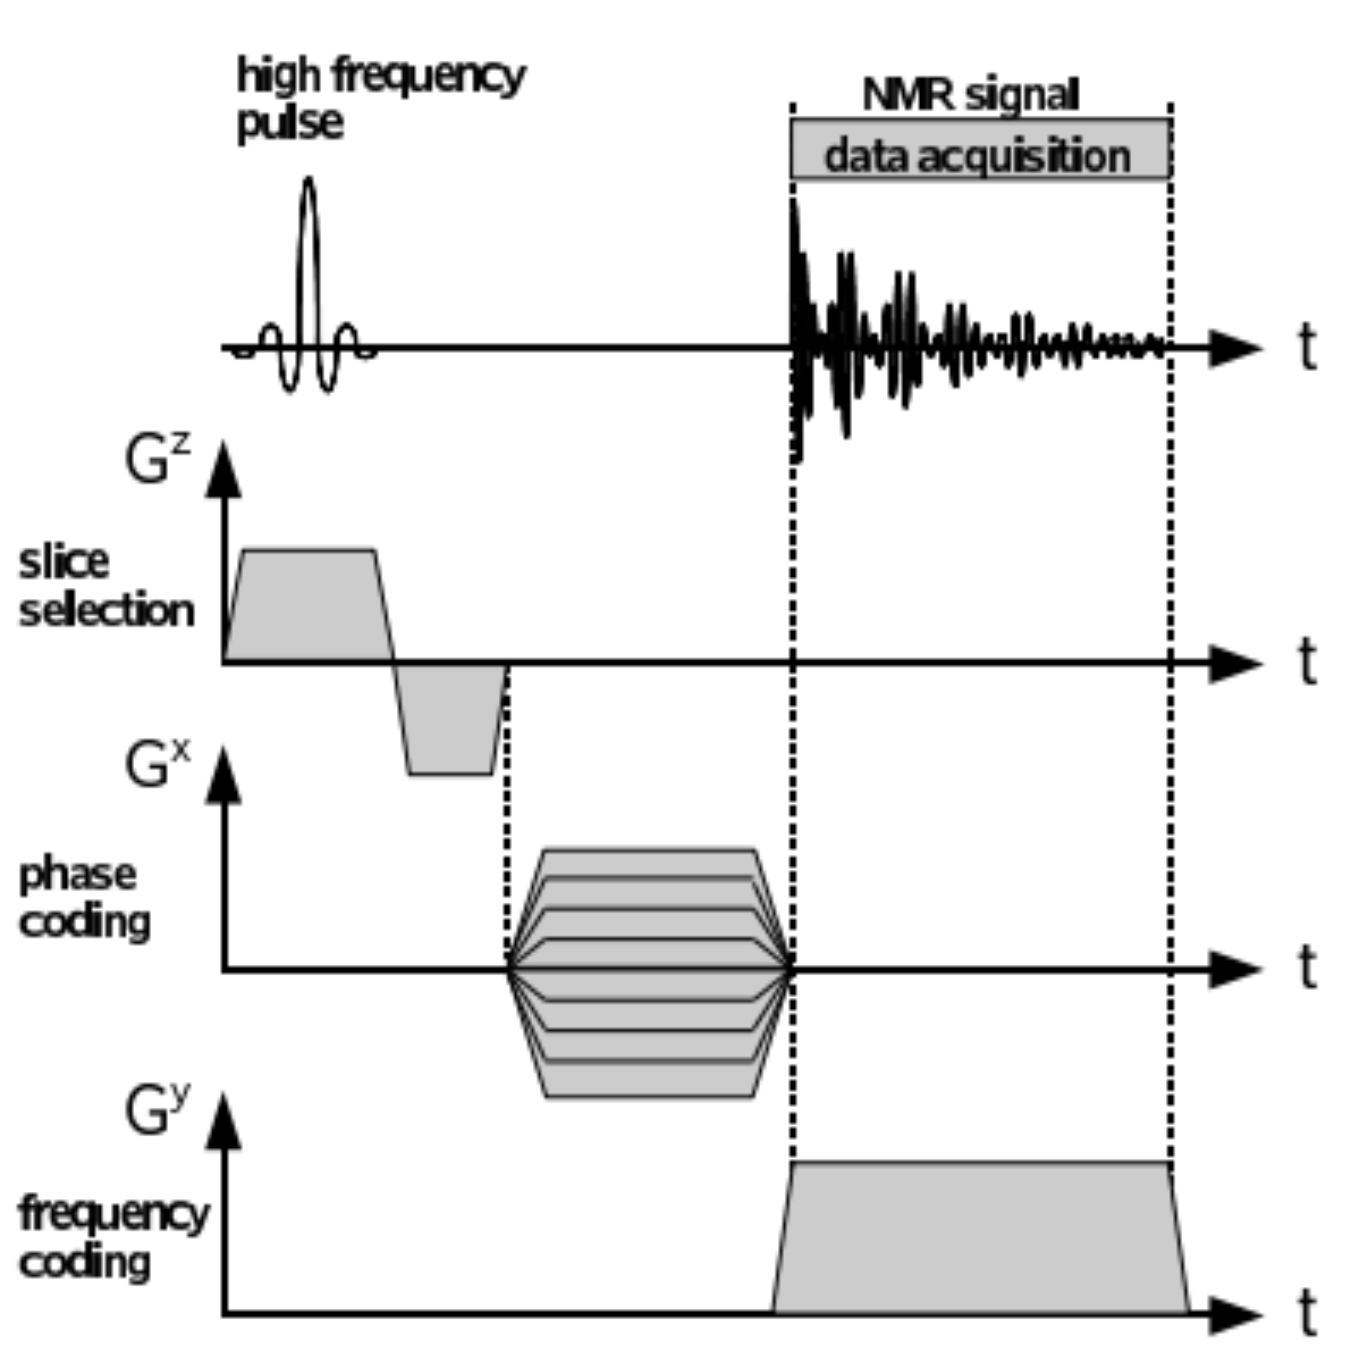
\includegraphics[scale=.1]{images//signal.png}
\end{frame}




%---------------
%Diskussion
%---------------
\section{Diskussion}
\begin{frame}{Fazit}
alles
\end{frame}

\begin{frame}{Anwendung}
haehd
\end{frame}